\documentclass{beamer}
\usetheme{Madrid}
\usepackage[utf8]{inputenc}
\usepackage[T1]{fontenc}
\usepackage{graphicx}
\usepackage{lmodern}

% Pour enlever le \institute du bas de page
% Rapetisser les noms et date etc dans le footer
\setbeamertemplate{footline}
{
  \leavevmode%
  \hbox{%
  \begin{beamercolorbox}[wd=.333333\paperwidth,ht=2.25ex,dp=1ex,center]{author in head/foot}%
    \
  \end{beamercolorbox}%
  \begin{beamercolorbox}[wd=.333333\paperwidth,ht=2.25ex,dp=1ex,center]{title in head/foot}%
    \usebeamerfont{title in head/foot}\insertshorttitle
  \end{beamercolorbox}%
  \begin{beamercolorbox}[wd=.333333\paperwidth,ht=2.25ex,dp=1ex,right]{date in head/foot}%
    \usebeamerfont{date in head/foot}\insertshortdate{}\hspace*{2em}
    \insertframenumber{} / \inserttotalframenumber\hspace*{2ex} 
   \end{beamercolorbox}}%
  \vskip0pt%
}

\AtBeginSection[]
{
	\begin{frame}
		\tableofcontents[currentsection,hideallsubsections]
	\end{frame}
}

\title{Soutenance TER : Moteur de Streaming}
\author{Kevin Bollini, Valentin Hirson, Thomas Hinsinger}
\date{4 Mars 2013}

\begin{document}
	\begin{frame}
		\titlepage
	\end{frame}

	%Plan
	\begin{frame}{Plan}
		\tableofcontents
	\end{frame}

	\section{Introduction}
		
		
	\section{Analyse et Conception}
	\subsection{Gestion de projet}
		\begin{frame}{Gestion de projet}
		Organisation :
			\begin{itemize}
				\item{Méthode agile}
				\item{Partage des tâches}
				\item{Développement incrémental}
			\end{itemize} \pause
			Collaboration :
			\begin{itemize}
				\item{Gestionnaire de versions}
				\item{Partage de documents}
				\item{Discussions (Mails / Instantanée)}
				\item{Édition collaborative}
			\end{itemize}
		\end{frame}

		\begin{frame}{Sprints}
			\begin{center}
				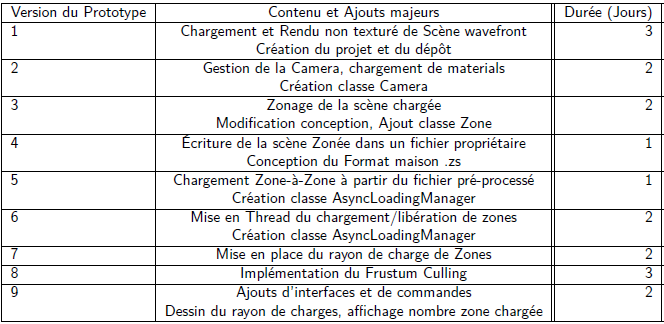
\includegraphics[scale=0.5]{images/recapProto.png} \\
				Récapitulatif des prototypes\\
			\end{center}
		\end{frame}

		\begin{frame}{Outils}
			\begin{alertblock}{Outils Techniques}
				\begin{itemize}
					\item Gestionnaire de versions : Subversion
					\item Integrated Development Environment : Monodevelop
					\item Discussions (Mails / Instantanée)
				\end{itemize}
			\end{alertblock}
			 \pause
			\begin{exampleblock}{Bibliothèque}
				\begin{itemize}
					\item OpenTK
				\end{itemize}
			\end{exampleblock}
		\end{frame}
	
	\subsection{Analyse}
		\begin{frame}{Diagramme de classes}
			\begin{center}
				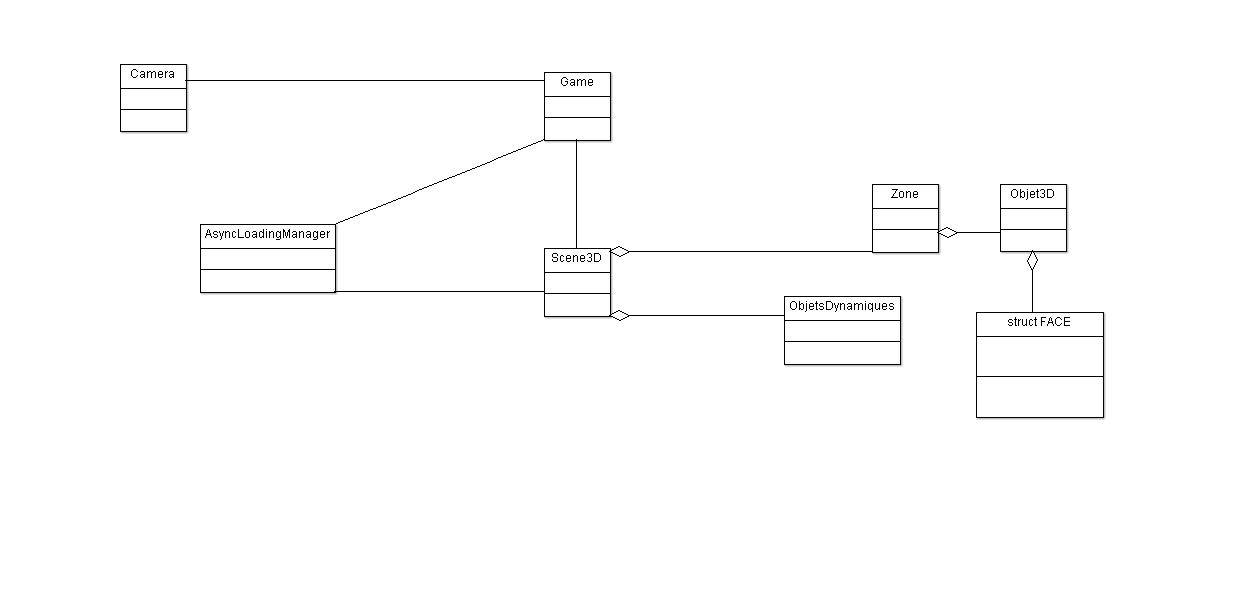
\includegraphics[scale=0.3]{Rapport/images/ClassDiagram.png} \\
				\tiny{Diagramme de classes\\} 
			\end{center}
		\end{frame}

	\section{Réalisation}
		\subsection{PréProcessing}
			
		\subsection{Chargement Asyncrone}
			\begin{frame}{Chargement Asyncrone}
			\begin{block}{Stockage des données}
				\begin{itemize}
					\item{Éléments Statiques}
					\item{Éléments Dynamique}
					\item{Textures et Materials}
				\end{itemize}
			\end{block}
			\pause
			\begin{exampleblock}{Chargement Asyncrone}
				\begin{itemize}
					\item{Thread dédié}
					\item{Pile de tâche : LIFO}
				\end{itemize}
			\end{exampleblock}
			\pause
		\end{frame}
		\begin{frame}{Classe Scene3D}
			\begin{center}
				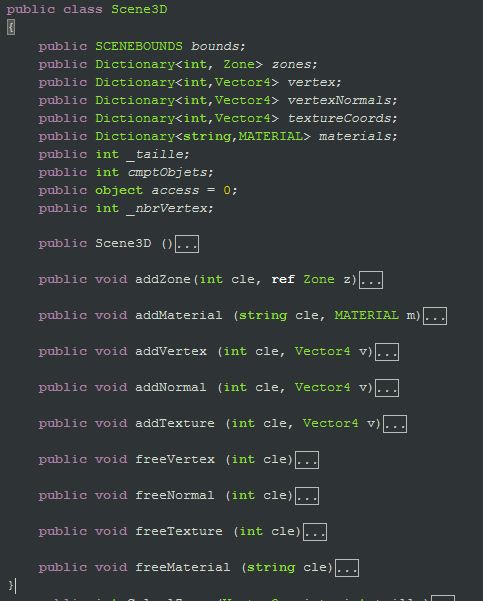
\includegraphics[scale=0.45]{images/extraitStockage.png} \\
				\tiny{Signature classe Scene3D\\} 
			\end{center}
		\end{frame}
		\subsection{Rendu}

	\section{DEMONSTRATION}

	\section{Discussion}
			
	
	

	\section{Conclusion}
		\begin{frame}{Conclusion}
			\begin{alertblock}{Difficultés}
				\begin{itemize}
					\item{Syncronisation}
					\item{Technologie}
				\end{itemize}
			\end{alertblock}
			\pause
			\begin{exampleblock}{Objectifs atteints}
				\begin{itemize}
					\item{Streaming}
				\end{itemize}
			\end{exampleblock}
		\end{frame}
		\begin{frame}{Ouverture}
			\begin{block}{Ouverture}
				\begin{itemize}
					\item Texture
					\item Level of Detail
					\item Objets Dynamiques
					\item Waypoints
				\end{itemize}
			\end{block}
		\end{frame}
	
	\begin{frame}
		\begin{center}
			\huge{Merci pour votre attention.} \\
			
\includegraphics[scale=0.32]{images/tux.png}
		\end{center}
	\end{frame}

\end{document}